\section{Analysis}

\subsection{Use Case analysis}

\subsubsection{Class Candidates}
In order to find potential class candidates, every noun of the detailed Use
Cases are found. These are potential candidates, and can be sorted to avoid
duplicates and candidates that won’t be turned into classes. Naturally, every
potential class for the entire system will not be found, as this only reflects
use cases. A potential class candidate such as MES (where Start and Stop
functionality would otherwise be implemented) will not be reduced to a single
class and is therefore not added to the list of class candidates.

The final list of classes, as well as a description of them, can be seen in
table \ref{table:class_candidates}.

\begin{table}[ht]
    \begin{tabularx}{\textwidth}{|>{\RaggedRight}p{4cm}|>{\RaggedRight}p{6cm}|>{\RaggedRight}X|}
    \hline
    \textbf{Class Candidate} & \textbf{Attributes}                                                                                                     & \textbf{Definition}                                                                    \\ \hline
    Batch                    & Id, type, product\_amount (total, defect, acceptable), amount (time), state (current, history), OEE, production\_speed, & A batch refers to a specific batch of products the brewery has made                    \\ \hline
    Product                  & Id, type, Ingredients,                                                                                                  & Product refers to the different options of beer to be produced                         \\ \hline
    Ingredient               & Name, id                                                                                                                & An ingredient refers to a specific ingredient. Products contain a list of ingredients. \\ \hline
    \end{tabularx}
    \caption{Potential class candidates}
    \label{table:class_candidates}
    \end{table}

\subsubsection{UML Analysis Diagram}
From the verb/noun analysis from the previous chapter, the UML analysis diagram
seen in figure \ref{figure:analysis_diagram}, can be generated. This diagram
shows the classes and attributes found in the requirements from the project
description.

\begin{figure}[ht]
	\centering 
	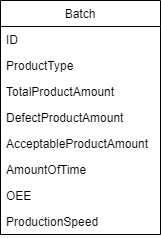
\includegraphics[scale=0.6]{images/diagrams/UML_Analysis_Diagram.drawio.png}
	\caption{UML Analysis diagram}
	\label{figure:analysis_diagram} 
\end{figure}

\subsection{Use Case Realisation}

\subsubsection{Sequence Diagrams}

\subsubsection{Operation Contracts}

\subsubsection{Updated UML Class Diagram}
